\chapter{Cases}
		\section{Case 1}
			Until this point the improvements were only run separated from each other (except the second improvement). However the final goal was to used them all in the simulator and check how it effects the outcome.
			\subsection*{Initial conditions}
			The initial conditions remained the same, except additional parameters were necessary to provide for the improvements. The initial conditions with the additional parameters can be found in Table \ref{tab:new_array}. The table contains the time intervals whenever a driver is not paying attention as well as the acceleration threshold values.
			\begin{table}[ht]
				\begin{center}
					\begin{tabular}{ |c|c|c|c| }
						\hline
						Id & ... & Time interval of driving without attention & $a_{\rm p,tr}$\\
						$[-]$ & & [s]& $\rm [m/s^2]$\\
						\hline
						1 & ... & 24-26 & 1.2 \\
						2 & ... & 0-2 & 1.2 \\
						3 & ... & 10-12 & 1.3 \\
						4 & ... & 0-3, 22-24, 25-25.5 & 1.3 \\
						5 & ... & 15-19 & 1.6 \\
						6 & ... & 15-16.5 & 1.6 \\
						7 & ... & 0-2 & 1.3 \\
						8 & ... & - & 1.1 \\
						9 & ... & 0-3 & 1.3 \\
						1 & ... & 0-4,15-18.5 & 1.7 \\
						\hline
					\end{tabular}
				\end{center}
				\caption{Initial conditions of Case 1}
				\label{tab:new_array}
			\end{table}
			\begin{figure}
				\centering
				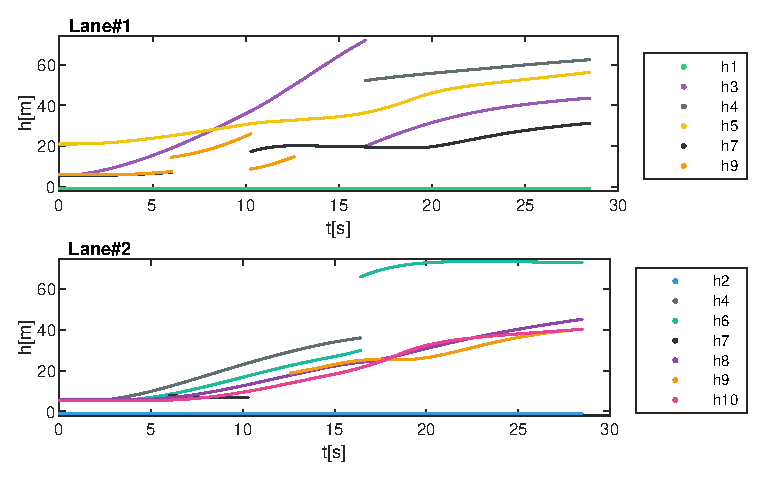
\includegraphics[width=0.8\textwidth]{eemobil/simh_case5}
				\caption{Traffic light case 1. Headway of the vehicles respect to their position in lanes}
				\label{fig:red_light_situationh2}
			\end{figure}
			\begin{figure}
				\centering
				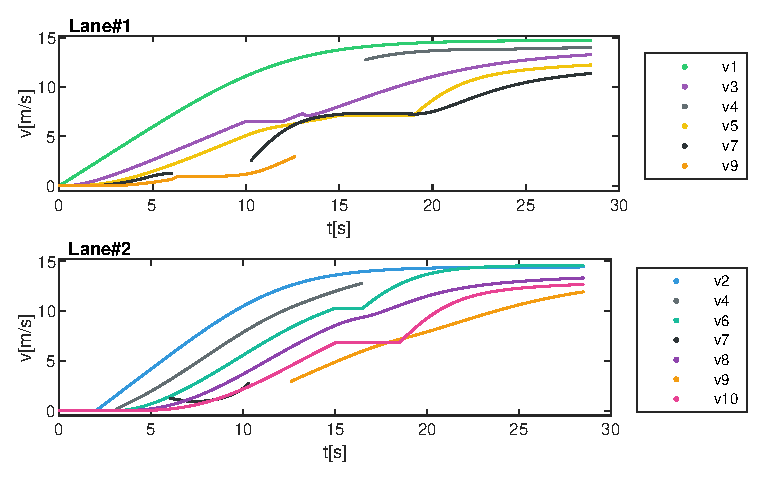
\includegraphics[width=0.8\textwidth]{eemobil/simv_case5}
				\caption{Traffic light case 1. Velocity of the vehicles respect to their position in lanes}
				\label{fig:red_light_situationv2}
			\end{figure}
			\begin{figure}
				\centering
				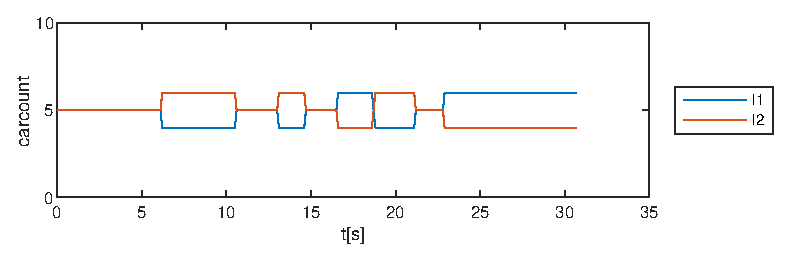
\includegraphics[width=0.8\textwidth]{eemobil/simcc_case5}
				\caption{Traffic light case 1. Number of cars in lanes }
				\label{fig:red_light_situationcc2}
			\end{figure}
			\subsection*{Summary of the result}
			The results can be seen on Figure \ref{fig:red_light_situationh2}, \ref{fig:red_light_situationv2} and \ref{fig:red_light_situationcc2}. The results shows that including all improvement the overall duration has increased to \casetime{5}from the original \casetime{1}seconds.
		\section{Case 2}
			Another interesting situation is that how an obstacle effects this simulation. E.g.: Place an obstacle into target line and see what is the outcome. Every other parameters of the simulation remained the same.
			\begin{figure}[ht]
				\centering
				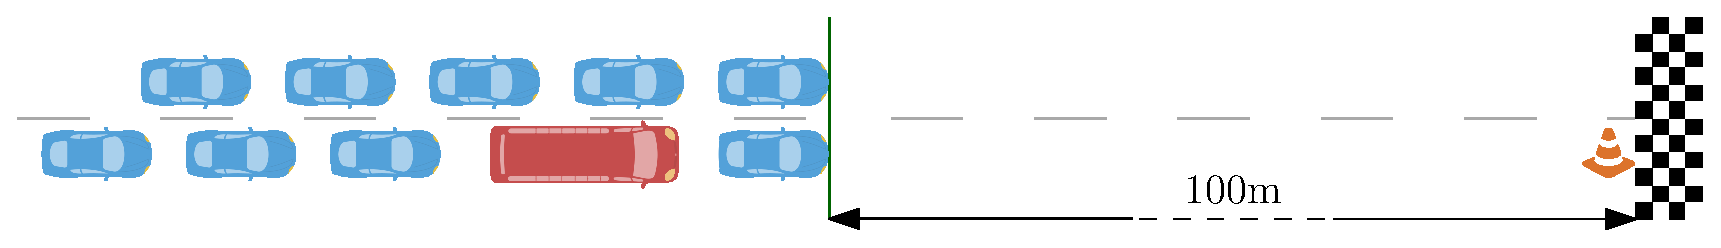
\includegraphics[width=\textwidth]{common/traffic_light_init_case2}
				\caption{Case 2 initial positions}
				\label{fig:traffic_light_init2}
			\end{figure}
			\begin{figure}[ht]
				\centering
				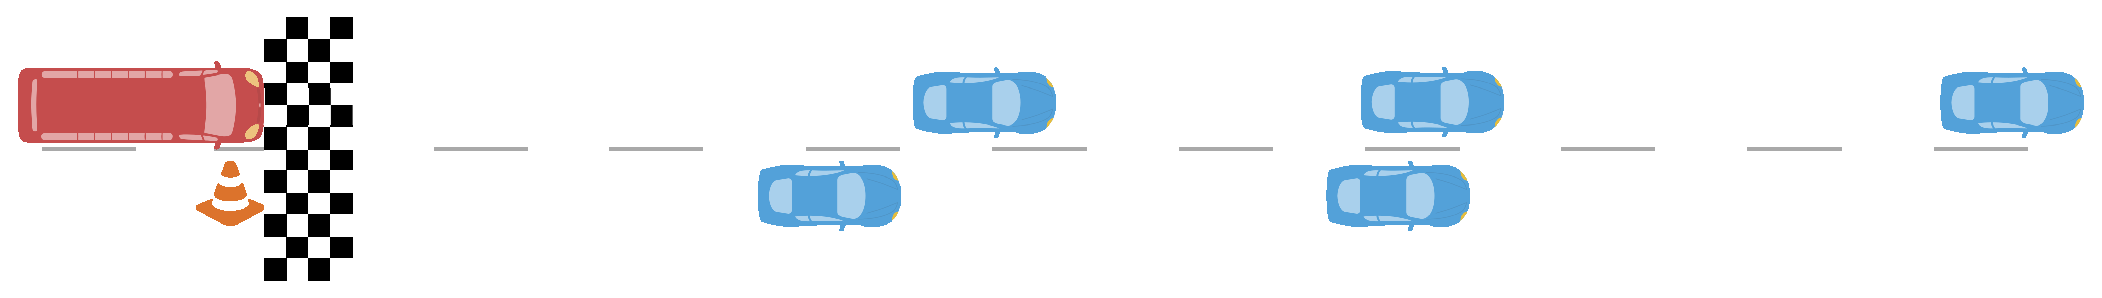
\includegraphics[width=\textwidth]{common/traffic_light_end_case2}
				\caption{Case 2 end postions}
				\label{fig:traffic_light_end2}
			\end{figure}
			\begin{figure}
				\centering
				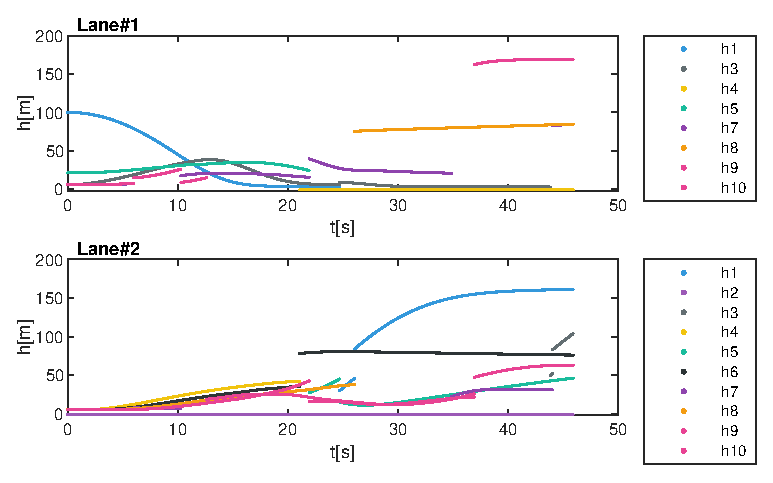
\includegraphics[width=0.8\textwidth]{eemobil/simh_case6}
				\caption{Traffic light case 2. Headway of the vehicles respect to their position in lanes}
				\label{fig:red_light_situationh3}
			\end{figure}
			\begin{figure}
				\centering
				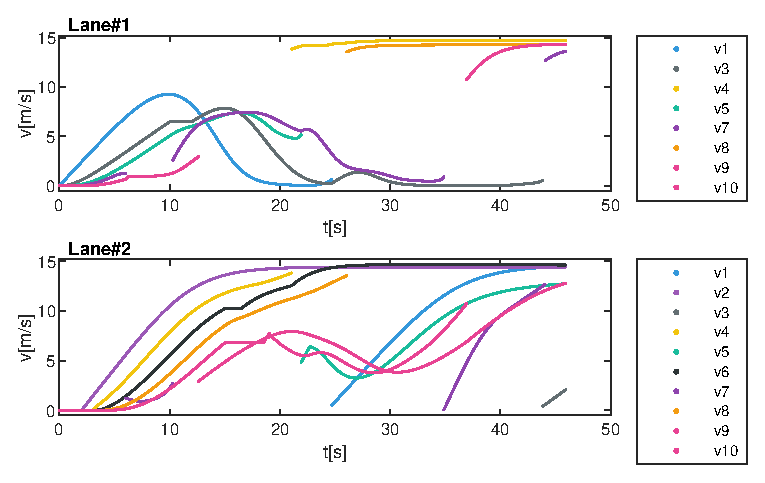
\includegraphics[width=0.8\textwidth]{eemobil/simv_case6}
				\caption{Traffic light case 2. Velocity of the vehicles respect to their position in lanes}
				\label{fig:red_light_situationv3}
			\end{figure}
			\begin{figure}
				\centering
				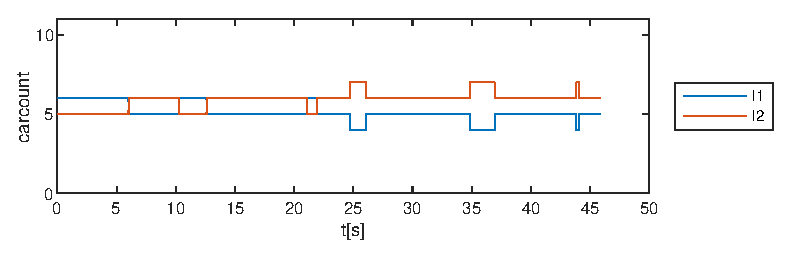
\includegraphics[width=0.8\textwidth]{eemobil/simcc_case6}
				\caption{Traffic light case 2. Number of cars in lanes }
				\label{fig:red_light_situationcc3}
			\end{figure}